\documentclass{extbook}[14pt]
\usepackage{multicol, enumerate, enumitem, hyperref, color, soul, setspace, parskip, fancyhdr, amssymb, amsthm, amsmath, bbm, latexsym, units, mathtools}
\everymath{\displaystyle}
\usepackage[headsep=0.5cm,headheight=0cm, left=1 in,right= 1 in,top= 1 in,bottom= 1 in]{geometry}
\pagestyle{fancy}
\lhead{}
\chead{Answer Key for Module\,11M\,-\,Modeling\,with\,Log\,and\,Exp\,Functions Version B}
\rhead{}
\lfoot{Summer\,C\,2020}
\cfoot{}
\rfoot{}
\begin{document}
\textbf{This key should allow you to understand why you choose the option you did (beyond just getting a question right or wrong). \href{https://xronos.clas.ufl.edu/mac1105spring2020/courseDescriptionAndMisc/Exams/LearningFromResults}{More instructions on how to use this key can be found here}.}

\textbf{If you have a suggestion to make the keys better, \href{https://forms.gle/CZkbZmPbC9XALEE88}{please fill out the short survey here}.}

\textit{Note: This key is auto-generated and may contain issues and/or errors. The keys are reviewed after each exam to ensure grading is done accurately. If there are issues (like duplicate options), they are noted in the offline gradebook. The keys are a work-in-progress to give students as many resources to improve as possible.}

\rule{\textwidth}{0.4pt}

51. The temperature of an object, $T$, in a different surrounding temperature $T_s$ will behave according to the formula $T(t) = Ae^{kt} + T_s$, where $t$ is minutes, $A$ is a constant, and k is a constant. Use this formula and the situation below to construct a model that describes the uranium's temperature, $T$, based on the amount of time t (in minutes) that have passed. Choose the correct constant $k$ from the options below.
Uranium is taken out of the reactor with a temperature of $200^{\circ}$ C and is placed into a $10^{\circ}$ C bath to cool. After 32 minutes, the uranium has cooled to $132^{\circ}$ C. 
The solution is $ k = -0.01384 $ 

\begin{enumerate}[label=\Alph*.] 
\item $ k = -0.01384 $ 

 * This is the correct option. 
\item $ k = -0.02384 $ 

 This uses $A$ as the initial temperature and solves for $k$ correctly. 
\item $ k = -0.02403 $ 

 This uses $A$ correctly but solves for $k$ incorrectly. 
\item $ k = -0.01545 $ 

 This uses $A$ as the initial temperature and solves for $k$ incorrectly. 
\item $ \text{None of the above} $ 

 If you chose this, please contact the coordinator to discuss why you believe none of the other answers are correct. 
\end{enumerate} 
 
\textbf{General comments:} The initial temperature is when $t = 0$. Unlike power models, that means $A$ is not the initial temperature!

-----------------------------------------------

52. Using the scenario below, model the situation using an exponential function and a base of $\frac{1}{2}$. Then, solve for the half-life of the element, rounding to the nearest day.
The half-life of an element is the amount of time it takes for the element to decay to half of its initial starting amount. There is initially 509 grams of element $X$ and after 12 years there is 127 grams remaining. 
The solution is $ \text{About } 1825 \text{ days} $ 

\begin{enumerate}[label=\Alph*.] 
\item $ \text{About } 2920 \text{ days} $ 

 This uses the correct model but a base of $e$ rather than $\frac{1}{2}$. 
\item $ \text{About } 4745 \text{ days} $ 

 This uses the correct model but solves for the exponential constant incorrectly. 
\item $ \text{About } 1825 \text{ days} $ 

 * This is the correct option. 
\item $ \text{About } 730 \text{ days} $ 

 This models half-life as a linear function. 
\item $ \text{None of the above} $ 

 Please contact the coordinator if you believe all the options above are incorrect. 
\end{enumerate} 
 
\textbf{General comments:} The model should be $A(t) = A_0 (\frac{1}{2})^{kt}$, where $A(t)$ is the amount after $t$ years, $A_0$ is the initial amount, and $k$ is decay constant. To find the half-life, you need to solve for $k$ by using the amount after $x$ years, then solve for the time $t$ when $A = \frac{A_0}{2}$. Your answer would be in years, so convert to days.

-----------------------------------------------

53. Determine the appropriate model for the graph of points below.
\begin{center} 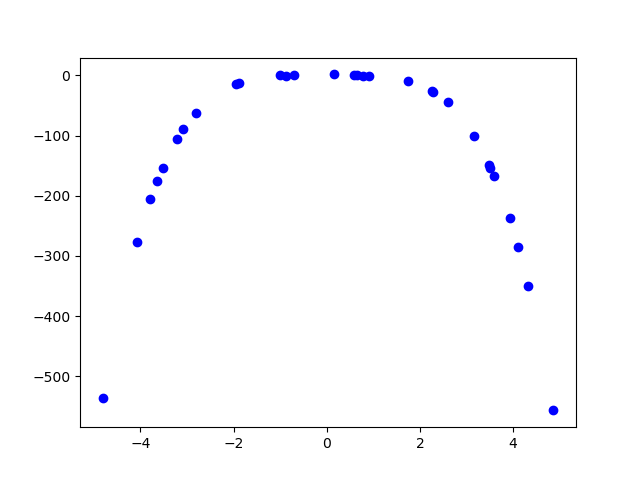
\includegraphics[width=0.3\textwidth]{../Figures/identifyModelGraph11B.png} \end{center} 

The solution is $ \text{None of the above} $ 

\begin{enumerate}[label=\Alph*.] 
\item $ \text{Exponential model} $ 

 For this to be the correct option, we want an extremely slow change early, then a rapid change later. 
\item $ \text{Logarithmic model} $ 

 For this to be the correct option, we want a rapid change early, then an extremely slow change later. 
\item $ \text{Non-linear Power model} $ 

 For this to be the correct option, we need to see a polynomial or rational shape. 
\item $ \text{Linear model} $ 

 For this to be the correct option, we need to see a mostly straight line of points. 
\item $ \text{None of the above} $ 

 For this to be the correct option, we want to see no pattern in the points. 
\end{enumerate} 
 
\textbf{General comments:} This question is testing if you can associate the models with their graphical representation. If you are having trouble, go back to the corresponding Core module to learn about the specific function you are having trouble recognizing.

-----------------------------------------------


\end{document}

